\documentclass[a4paper]{article}

\usepackage[T1]{fontenc}
\usepackage[utf8]{inputenc}
%\usepackage[ngerman]{babel}
\usepackage{times, graphicx, currvita, hyperref, longtable, float, caption, subcaption}
\usepackage{amsmath,amsfonts,amssymb, amsthm}%, dsfont, bbm, mathtools, stmaryrd}
\usepackage{fancyhdr}
\usepackage{color}
% \usepackage{pgf}
\usepackage{tikz}
\usetikzlibrary{patterns,decorations.markings,arrows,calc}
\usepackage[english]{babel}
\usepackage{paralist}
\usepackage{algorithm}
\usepackage{algpseudocode}%should also load algorithmicx
\usepackage{hyperref}

% \usepackage{wasysym}	% verschiedene Symbole, siehe http://rpi.edu/dept/arc/training/latex/LaTeX_symbols.pdf
\usepackage{marvosym}
\graphicspath{{Bilder/}}

\theoremstyle{definition}
\newtheorem{definition}{Definition}[section]
\newtheorem*{Def1}{Definition}
\newtheorem*{ex}{Example}

\newtheoremstyle{Tobi}{10pt}{}{}{}{\bf}{ }{\newline}{}
% die parameter sind: {name}{platz drueber}{platz drunter}{schriftart text}{einrueckung}{schriftart kopf}{Punktierung des Kopfes}{Platz zwischen kopf und text}

\theoremstyle{Tobi}
\newtheorem{prop}[definition]{Proposition}
\newtheorem*{Pro}{Proposition}
\newtheorem{theorem}[definition]{Theorem}
%\newtheorem*{le}{Lemma}
\newtheorem{lemma}[definition]{Lemma}
\newtheorem{cor}[definition]{Corollary}
\newtheorem*{conj}{Conjecture}
\newtheorem{obs}[definition]{Observation}

% \theoremstyle{remark}
% \newtheorem*{que}{Questions}
% \newtheorem*{claim}{Claim}
% \newtheorem*{note}{Note:}
% \newtheorem*{remark}{Remark}


\newcommand{\R}{\mathbb{R}}
\newcommand{\N}{\mathbb{N}}
% \newcommand{\F}{\mathbb{F}}
% \newcommand{\1}{\mathbbm{1}}
\newcommand{\Rn}{\mathbb{R}^n}
% \newcommand{\La}{\mathcal{L}}
% \newcommand{\D}{\mathcal{D}}
\newcommand{\Om}{\Omega}
\newcommand{\pa}{\partial}
\newcommand{\C}{\mathcal{C}}
\newcommand{\ph}{\varphi}

\setlength{\parindent}{0pt}

%define tikz picture elements setting global here as style for all tikz pictures
%this is to set arrow in middle of lines
\tikzset{->-/.style={decoration={markings, mark=at position .5 with {\arrow{#1}}},postaction={decorate}}}
\tikzset{vertex/.style={circle,fill=black!40}}
\tikzset{source/.style={circle,draw=green,fill= green!20}}
\tikzset{sink/.style={circle,draw=red,fill =red!20}}
\tikzset{every picture/.append style={scale=2.5}}%maybe better set locally?
\tikzset{edge/.style={semithick, solid}}%could also do dashed, dotted, double...
\tikzset{arc/.style={->-, semithick}}
\tikzset{fatarc/.style={very thick, ->-={latex}}}
\tikzset{edgeflow/.style={line width=3pt, #1!40}} %rounded corners funzt nicht?
\tikzset{arcflow/.style={->-, line width=3pt, #1!40}}
\tikzset{edgeflow/.default=blue}
\tikzset{arcflow/.default=blue}
\tikzset{->-/.default=stealth}
\tikzset{curvedarc/.style={arc, bend angle = 10, bend right}}
\tikzset{curvedarcflow/.style={arcflow, bend angle = 10, bend right}}
% \begin{figure}[h!]
% \centering
% \begin{tikzpicture}
% \node (s) at (0,0)[vertex, label=s]{};
% \draw[arcflow] (s)--(3)--(t);
% \end{tikzpicture}
% \caption{}
%  \label{bild:}
% \end{figure}

\begin{document}

\title{Entwurf MA - Bounds for Acyclic Network Flows}

\author{Tobias Buchwald}
% \maketitle

%\large{Bachelorarbeit bei Prof. Dr. Stefan Felsner}


\begin{center} 

\Huge{Bounds for Acyclic Network Flows}\\ \vspace{12 cm}
\Large{Masterarbeit\\ bei Prof. Dr. Thorsten Koch}\\ \vspace{1cm}
\large{Vorgelegt von Tobias Buchwald}\\
\large{am Fachbereich Mathematik der \\Technischen Universit\"at Berlin}\\
\vspace{2cm}
\large{Berlin,  \today}

\end{center} 


\textbf{Erkl\"arung}\\

Hiermit versichere ich an Eides statt, dass ich die vorliegende Masterarbeit selbst\"andig und eigenh\"andig sowie
ausschlie\ss lich unter Verwendung der aufgef\"uhrten Quellen und Hilfsmittel angefertigt habe. \\


Berlin, den \today
\newline

\rule[-0.2cm]{10cm}{0.5pt}

\textsl{Tobias Buchwald} 
\newpage

\tableofcontents
\newpage
\section*{Zusammenfassung}%TODO deutsche Zusammenfassung der Arbeit (ist vorgabe der studienordnung)
Die vorliegende Arbeit beschäftigt sich mit dem Problem, den maximalen azyklischen Fluss in einem 
Flussnetzwerk mit gegebenen Kapazitäten sowie Ein- und Ausspeisungen an Quellen und Senken zu finden. 

Eine möglichst gute Schranke für den azyklischen Fluss ist ein Baustein für gutes Preprocessing 
für die Nominierungsvalidierung in Gasnetzen. Gasfluss ist druckinduziert und daher (abgesehen von Verdichterstationen) 
azyklisch. Es ist möglich, einen Fluss mit minimalen Kosten in einem Netzwerk mit einem negativen Gewicht auf der 
Kante, deren Fluss zu maximieren ist, zu berechnen um den Flusswert der Kante zu maximieren. Dieser Ansatz führt 
allerdings zu wesentlich schwächeren Schranken als der azyklische (in der Tat ist 
die Lücke zu azyklischen Flussschranken unbeschränkt). Gleichzeitig ist erzwingen von Azyklizität des Flusses vor allem 
in dem Fall der Extrema des Flusswertes interessant. Einen beliebigen azyklischen Fluss kann man in einem Netzwerk 
immer erhalten wenn man irgendeinen Fluss gegeben hat. Dieser erfüllt aber nicht die Maximalitätsbedingungen.


Die Arbeit ist folgendermaßen strukturiert: Das Problem und wichtige mathematische Grundlagen werden zunächst definiert 
und Bezüge zu verwandten algorithmischen Problemen hergestellt. 
Für das Problem des kostenminimalen Flusses mit negativen Gewichten wird NP-Vollständigkeit bewiesen und eine Reduktion 
dieses Problems angegeben. 
Zur Lösung des Azyklischen Flussschrankenproblems werden verschiedene Modelle als (Quadratic) 
Mixed Integer Program vorgestellt. Es werden Ungleichungen zur Erzwingung azyklischen Flusses aus einem der Modelle 
untersucht und Kriterien für deren Redundanz/benötigte Aanzahl angegeben und bewiesen. Ein theoretisches Modell für ein 
pfadbasierte Flussaugmentierung wird untersucht und eine Heuristik für das Problem entwickelt.
Die verschiedenen Lösungsansätze wurden implementiert und werden in ihren Ergebnissen, Auswirkungen auf
die Modellgröße im Preprocessing und Laufzeitverhalten auf Testinstanzen verglichen.
\newpage
\section{Introduction} \subsection{Motivation and Outline}
Today more and more real-world problems in the areas of simulation and optimization are solved by mathematical and 
computational methods. A growing number of these problems can be solved without problems, i.e. even huge instances give 
an optimal or near optimal solution within seconds. Still, there remain problems that even on modern computers are hard 
to solve. For these problems it is important to find ways to increase the efficiency of the algorithms. 

The topic of this thesis arises from the computation of flow in natural gas networks, which is currently developed 
in the FORNE Project in a cooperation of OGE with universities and research insitutes including ZIB.
%TODO genaueres zu FORNE? genaueres zum aufbau des Gasnetzes?
The flow of natural gas in a network is described by nonlinear equations and depends on many parameters, which makes 
the problem hard to solve. If we can find good upper and lower bounds for the flow on an arc during the preprocessing, 
we can hope to improve the behavior of the nonlinear solver by giving these tigther bounds. 

The flow is induced by pressure differences, so in reality there can't be cyclic flow (if we exclude compressor 
stations). Without the condition of acyclic flow, it is sufficient to run a standard min-cost-flow algorithm where the 
maximized arc $e$ gets weight $w_e = -1$ and all others are 0. However, the arising bounds are far from optimal. If arc 
$e$ is contained in any cycle we could decrease the cost by pushing more and more flow around this cycle until the arcs 
capacity is at its limits.

This master thesis will deal with the problem of finding a network flow with no directed cycles (acyclic flow), which at 
the same time maximizes the amount of flow on a specified arc $e$ of the network. We will discuss the complexity, an 
exact algorithm based on a mixed integer program with separation of inequalities that forbid cycles and also a heuristic 
approach that yields results much faster (but not optimal).%TODO am ende genauer schreiben was wirklich gemacht wurde

% \subsection{The gas flow problem}
% Although it is mainly the motivation, not really the topic of this thesis, we want to briefly introduce the gas 
% transport problem. For more a detailed description we refer to LINK 
% %TODO link auf ein entsprechendes ZIB-paper? Nee, Jesco meinte soll nicht so rein 
% 

\newpage
% \subsection{Motivation}
Natural gas is one of the most common ressources of energy in germany and makes up more than 20 percent of energy 
consumption. Most of this gas is produced in ressource-rich countries like Russia or Norway and transported to Germany 
through special pipelines. 
%TODO wie sollte ich das projekt am besten referenzieren?
This thesis evolved from a joint research project of the Konrad Zuse Zentrum fuer Informationstechnik Berlin (ZIB) with 
Open Grid Europe (OGE) who operate the largest network of gas pipelines in germany. 
A general overview over the work done at ZIB on the gas network planning in this project is given in 
\cite{FuegenschuhGeisslerGollmeretal.2013}. The problem of finding settings for all active components of the network 
such that given (static) demands and supplies can be sent through the network with respect to all constraints is the 
\textit{nomination validation} problem. A description of the model used and work done at ZIB for the nomination 
validation problem can be found in \cite{PfetschFuegenschuhGeissleretal.2012}. 

The flow of gas through a pipeline network is determined by physical conditions such as pressure and temperature. 
Pressure can be increased in compressor stations and controlled by elements like valves. Pressure loss along a pipe is 
described by ordinary differential equations. 

The computation of such a physically exact flow is difficult due to numerical and algorithmical reasons. Good 
preprocessing routines can help a lot by reducing the domains and model sizes before the main computation is started.

Since the flow of gas in the network is always determined by pressure differences and flow is always going from higher 
pressure to lower pressure we know that flow in the network in general has to be acyclic. The only exception of this 
rule is a compressor station. While  active compressor stations increase
pressure it is possible that they cause cyclic flow. But of course in real gas networks a compressor station would 
normally be placed at a point where it has the highest impact. This is naturally at a place where it is unlikely to 
waste energy by sending flow on a cycle. The pressure would rather be controlled by resistors, valves and control valves 
in order to avoid cycing. So we will assume that the acyclic flow model is reasonable for the gas flow problem.\\

%erklärung warum wir engere Bounds brauchen können
The bounds are expected to be useful for two things in the solving process of the nomination validation problem 
described in \cite{PfetschFuegenschuhGeissleretal.2012}. If we have stronger bounds on the flow values in the network, 
it might improve the models that solve the actual nomination validation problem. 
%TODO detaillierter! Erst das Modell mit dem MIP beschreiben und dass es durch kleinere Intervalle die Zahl der vars 
%verringert
For the MILP approach described in \cite{PfetschFuegenschuhGeissleretal.2012} a linearization of the 
nonlinear model is computed. If the bounds are smaller or flow is even fixed to a specific value, the interval to be 
linearized is smaller. The smaller the interval, the less variables are needed. A small model might improve the running 
time and solvability of the model.

We also hope for improvements on the outer approximation with spatial branching approach. Here improved bounds could 
result in a stronger relaxation and thereby make solving the problem faster. \\
% TODO das MINLP beschreiben und wie sich im MINLP die Modellgroesse verkleinert?

So to have good bounds and reduce problem size is a goal set in order to reduce the overall running time of the 
nomination validation computations. To achieve this it is necessary to find the bounds quickly. This is why we also 
present relaxations/heuristics for the acyclic flowbound problem. The effects of the bounds on the MILP model reduction 
are shown in the last section of this thesis.



% We simplified the problem by assuming that there are no compressor stations or at least they do not cause cyclic flow. 
% At the same time we just ignore the physical properties of the gas. We do not compute or take care of any gas density, 
% pressure or possible pressure loss. Pressure is only used to justify the assumption of acyclicity. This abstraction is 
% justified by the fact that it is weaker than the original problem which also has to fulfill the flow conditions we use. 
% The bounds are only needed for preprocessing and to improve the model size in the end. 

\subsection{Related Work}
The diploma thesis of Thea Göllner \cite{DiplomarbeitTheaGoellner} describes preprocessing techniques for stationary gas 
network optimization models. This is the same model as the one we use here. In her thesis she also describes an 
algorithm for determining flow directions on the arcs of the network and determines cases in which we can fix the flow 
direction even on arcs contained in cycles of a certain kind. To achieve this she makes use of the acyclicity property 
of gas flow as well. 
Fixing a flow is basically saying that the lower flow bound in one direction is zero. Thus her work is a special case 
of the much more general approach on preprocessing acyclic bounds we have in here. The fixing of flow directions that 
she proposes works on induced paths of the network and on cycles where flow can only be coming in from one side. 
She also shows the restrictions of this approach and says that for many cases it is necessary to take pressure or flow 
quantity into account in order to see if one can fix the direction variable. 

Here we aim at computing more general acyclic flow bounds. So we can not only fix the direction of flow in some special 
cases but also give upper bounds on possible flow and bounds in cases were it is not clear which direction flow has to 
take. It still yields flow directions in the cases described. But in practice a combination of our models with the 
flow direction fixing Göllner did could improve runtime and quality, because for big networks we can only use heuristic 
algorithms in practice.

% \newpage
\subsection{Basic Notation and Definitions}% Als Referenz und Grundlage fuer die Definitionen nutze ich das Lehrbuch Combinatorial Optimization:Theory and 
%Algorithms von Bernhard Korte u Jens Vygen - definiere die wichtigsten Sachen aber erstmal auch selbst

Since there are many definitions, which may differ slightly, we want to introduce now the basic notation and 
definitions that we use throughout this thesis. The definitions in this chapter are mainly taken from the textbook 
about combinatorial optimization from Korte and Vygen \cite{KorteVygenCombOpt2007}.

An undirected graph is a triple (V, E, $\Psi$), where $V$ and $E$ are finite sets and
$\Psi: E\to \{X \subseteq V: |X| = 2\}$. 
A directed graph or digraph is a triple $(V, E, \Psi)$,
where $V$ and $E$ are finite sets and $\Psi : E \to \{(v, w) \in V \times V : v \neq w\}$. In this thesis by a
graph we mean normally the directed graph. If we talk about undirected graphs it will be stated 
explicitly. The elements of $V$ are called vertices, the elements of $E$ are the edges. Edges of undirected graphs can 
also be called arcs to make clear that they are directed.

Two edges $e, e'$ with $\Psi(e) = \Psi ( e')$ are called parallel. Graphs without parallel
edges are called simple. For simple graphs we usually identify an edge $e$ with its
image $\psi(e)$ and write $G = (V(G), E(G))$, where $E(G) \subseteq \{X \subseteq V(G) : |X| = 2\}$
or $E(G) \subseteq V(G) \times V(G)$. We often use this simpler notation even in the presence
of parallel edges, then the ``set'' $E (G)$ may contain several ``identical'' elements. In this thesis all graphs 
are considered simple if nothing different is said. %TODO rausnehmen falls gar keine parallelen Kanten gebraucht werden
$|E(G)|$ denotes the number of edges, and for two edge sets $E$ and $F$ we always
have $|E \cup F | = |E | + |F |$ even if parallel edges arise.

We say that an edge $e = \{v, w\}$ or $e = (v, w)$ joins $v$ and $w$. In this case, $v$ and $w$ are adjacent. $v$ is a 
neighbour of $w$ (and vice versa). $v$ and $w$ are the endpoints of $e$. If $v$ is an endpoint of an edge $e$, we say 
that $v$ is incident with $e$. 
In the directed case we say that $( v, w)$ leaves $v$ and enters $w$, $v$ is the tail and $w$ is the head of the arc 
$e$. Two edges which share at least one endpoint are called adjacent.

For a digraph $G$ we sometimes consider the underlying undirected graph, i.e. the undirected graph $G'$ on the same 
vertex set which contains an edge $\{v, w\}$
for each edge $(v, w)$ of $G$. We also say that $G$ is an orientation of $G'$.
A subgraph of a graph $G = (V(G), E(G))$ is a graph $H = (V(H), E(H))$
with $V(H) \subset V(G)$ and $E(H) \subset E(G)$. We also say that $G$ contains $H$. $H$ is an
induced subgraph of $G$ if it is a subgraph of $G$ and $E (H) = \{ \{x, y\} \textrm{ resp. } (x, y) \in
E(G) : x, y \in V(H)\}$. Here $H$ is the subgraph of $G$ induced by $V(H)$. We also
write $H = G[V(H)]$. A subgraph $H$ of $G$ is called spanning if $V(H) = V(G)$.
If $v \in V(G)$, we write $G- v$ for the subgraph of $G$ induced by $V(G) \setminus {v}$.
If $e \in E(G)$, we define $G- e := (V(G), E(G) \setminus \{e\})$. Furthermore, the addition
of a new edge $e$ is abbreviated by $G + e := (V(G), E(G) \cup {e})$. If $G$ and $H$
are two graphs, we denote by $G + H$ the graph with $V(G +H)= V(G) \cup V(H)$
and $E(G +H)$ being the disjoint union of $E(G)$ and $E(H)$ (parallel edges may arise).

For a graph $G$ and $X, Y\subseteq V(G)$ we define $E(X, Y) := \{\{x, y\} \in E(G) : x \in
X \setminus Y, y \in Y \setminus X\}$ resp. $E^+(X, Y) := \{(x, y) \in E(G) : x \in X\setminus Y, y \in Y \setminus 
X\}$.
For undirected graphs $G$ and $X \subseteq V(G)$ we define $\delta(X) := E(X, V(G) \setminus X)$. The
set of neighbours of $X$ is defined by $ \Gamma(X) := \{v \in V(G) \setminus X : E(X, \{v\})  \neq \emptyset\}$.
For digraphs $G$ and $X \subseteq V(G)$ we define $\delta^+(X) := E^+(x, V(G) \setminus X)$, $\delta^-(x) :=
\delta^+(V(G) \setminus X)$ and $\delta(X) := \delta^+(x) \cup \delta^-(x)$. We use subscripts (e.g. $\delta_G(X)$) to
specify the graph $G$ if necessary.

For singletons, i.e. one-element vertex sets $\{v\} (v \in V(G))$ we write $\delta(v) :=
\delta(\{v\})$, $\Gamma(v) := \Gamma(\{v\}), \delta^+(v) := \delta^+(\{v\})$ and $\delta^-(v) := \delta^-(\{v\})$. The 
degree of a vertex $v$ is $|\delta(v)|$, the number of edges incident to $v$. In the directed case, the
in-degree is $|\delta^-(v)|$, the out-degree is $|\delta^+(v)|$, and the degree is $|\delta^+(v)|+ |\delta^-(v)|$.
A vertex $v$ with zero degree is called isolated. A graph where all vertices have
degree $k$ is called $k$-regular.

An edge progression $W$ in $G$ is a sequence $v_1, e_1, v_2, \dots , v_k, e_k, v_{k+1}$ such that $k \ge 0$,
and $e_i = (v_i, v_{i+ 1}) \in E(G)$ resp. $e_i = \{v_i, v_{i+1}\}\in E(G)$ for $i = 1, \dots , k$. If in
addition $e_i \ne e_j \,\forall\, 1 \le i < j \le k$, $W$ is called a walk in $G$. $W$ is closed if
$v_1 = v_{k+1}$. A path is a graph $P = (\{v_1, ... , v_{k+1}\}, \{e_1, ... , e_k\})$ such that $v_i \ne v_j$ for
$1 \le i < j \le k + 1$ and the sequence $v_1 , e_1 , v_2, \dots , v_k, e_k, v_{k+1}$ is a walk. $P$ is
also called a path from $v_1$ to $v_{k+1}$ or a $v_1 - v_{k+1}$-path. $v_1$ and $v_{k+1}$ are the endpoints
of $P$. By $P_{[x,y]}$ with $x, y \in V(P)$ we mean the (unique) subgraph of $P$ which is
an $x-y$-path. Evidently, there is an edge progression from a vertex $v$ to another
vertex $w$ if and only if there is a $v-w$-path.

A cycle is a graph $(\{v_1, \dots , v_k\}, \{e_1, \dots, e_k\})$ such that the sequence $v_1, e_1, v_2, 
\dots , v_k,e_k,v_1$ is a (closed) walk and $v_i \ne v_j$ for $1 \le i < j\le k$.
An easy induction argument shows that the edge set of a closed walk can be
partitioned into edge sets of cycles.

The length of a path or cycle is the number of its edges. If it is a subgraph
of $G$, we speak of a path or cycle in $G$. A spanning path in $G$ is called a
Hamiltonian path while a spanning cycle in $G$ is called a Hamiltonian cycle
or a tour. A graph containing a Hamiltonian cycle is a Hamiltonian graph.
For two vertices $v$ and $w$ we write $dist(v, w)$ or $dist_G (v, w)$ for the length of
a shortest $v-w$-path (the distance from $v$ to $w$) in $G$. If there is no $v-w$-path at all,
i.e. $w$ is not reachable from $v$, we set $dist(v, w) := \inf$. In the undirected case,
$dist(v, w) = dist(w, v)$ for all $v, w \in V(G)$.

We shall often have a cost function $c : E(G) \to \R$. Then for $F \subseteq E(G)$ we
write $c(F) := \sum_{e\in F} c(e)$ (and $c(\emptyset) = 0$). This extends $c$ to a modular function
$c : 2^{E(G)}\to \R$. Moreover, $dist_{(G,c)}(v, w)$ denotes the minimum $c(E(P))$ over all
$v-w$-paths $P$ in $G$.

\newpage
\section{The Acyclic Flowbound Problem}We already described the gas flow problem, where the motivation for this thesis came from. Here we want to define the 
problem as a general combinatorial flow problem with specific contraints. We will also give the formulation as a Mixed 
Integer Program (MIP) and as well some natural relaxations, which might be easier to solve.

We will represent our originally undirected graph by a directed graph where flow is allowed to go over edges backward 
and forward as well. This allows us to specify directions forward and backward on every edge in a consistant way. 


\begin{definition}
 Let $G=(V,A)$ be a directed Graph and $e \in A$ a specific arc of $G$. For every vertex $v\in V$ let there be a 
prescribed range for the amount of flow demand $[d_l(v), d_u(v)]\subset \R \setminus \{0\}$. Vertices with demand 
values greater than 0 are sinks, vertices with negative demand value are sources. The flow demands are assumed to be 
balanced on their (absolute) higher bound values 
$$\sum_{v \in V\textrm{ sink}}d_u(v)-\sum_{v \in V\textrm{ source}}d_l(v)=0$$ 
%TODO am ende kontrollieren, dass demands (was positiv, was negativ) konsistent verwendet wurde!

Let there be a capacity function $c:A\to \mathcal{P}(\R), \, c(a)=[c_l(a), c_u(a)],\, c_l(a)\le 0 \le c_u(a) \, \forall 
a\in A$, and a flow  $f: A\to \R $ with $c_l(a)\le f(a)\le 
c_u(a)\, \forall a\in A$ and $\sum_{a\in \delta^+(v)}f(a)-\sum_{a\in\delta^-(v)}f(a)+d(v) = 0 \, \forall v\in V$.\\
We call this flow a \textit{feasible network flow on G}.
\end{definition}

The standard definition of Flow Problems has fixed demand values $d(v)=const$ instead of an interval. These two 
definitions are equivalent in the way that you can transform them into each other easily in polynomial time. Obviously 
we can see fixed demands $d(v)$ as intervals with $d_l(v)=d_u(v)=d(v)$ consisting of only one point $[d(v), d(v)]$. The 
other way around we use a construction that adds only one node and $|\{v\in V| d_u(v)<0\}|+|\{v\in V| d_l(v)>0\}|$ arcs 
to the network.
\begin{prop}
 There is a (linear time) transformation from the flow problem with demand intervals on the vertices to the standard 
flow problem with fixed demands. 
\end{prop}
\begin{proof}
 Given a graph $G=(V,A)$ with demand intervals at the entries and exits, we construct a graph $G'=(V',A')$ as follows:
 $$V' := V\cup \{z\} \textrm{, and } A' := A\cup \{ (v,z)| d_u(v)<0 \}\cup\{ (z,v)|d_l(v)>0\}$$ On $G'$ we then have 
to redefine the arc capacity and node demands: 
$$c':A\to \mathcal{P}(\R)  \,, c'(a)= c'(u,v) = \begin{cases} \{x|x\in [0,d_u(u)-d_l(u)]\} &\textrm{if }v=z\\ 
\{x|x\in [0,d_u(v)-d_l(v)]\}&\textrm{if }u=z\\ \{x|x\in[c_l(a), c_u(a)]\} &\textrm{else } \end{cases}
$$ 
The node demands now are 
$$ d'(v)=\begin{cases} d_l(v) & \textrm{if v is source, i.e. }d_u(v)<0\\
         d_u(v) &\textrm{if v is sink, i.e. }d_u(v)>0
        \end{cases}
$$
If we compute a solution of the flow problem on $G'$ and restrict the flow to the arcs of $G$, we get the solution of 
the problem on $G$ that respects the demand intervals:\\ 
We call the demands in the solution restricted to arcs of $G$ $d^s$ and have $ d^s(u)=d'(u)+f'((u,z))$. The flow balance 
constraints in normal nodes 
(nodes with demand 0) do not change at all, since the only new node $z$ is not in their neighborhood. All vertices that 
are sources or sinks (per definition thy cannot be both at the same time) have $z$ as neighbor. The flow balance on a 
source $u$ before and after restriction to $G$ differs only by the flow on the artificial arc $(u,z)$. This flow 
$f'((u,z))$ is in the capacity range $[0,d_u(u)-d_l(u)]$. Hence for sources $u$ ($d'(u)<0$) with 
$d^s(u)=d'(u)+f'((u,z))$ we can conclude for the demands $d^s(u)$ of the solution restricted to $G$ 
$$d_l(u)\le d^s(u)=d'(u)+f'((u,z))=d_l(u)+\underbrace{f'((u,z))}_{0\le f'((u,z))\le d_u(u)-d_l(u)} \le d_u(u)$$
and as well for sinks ($d'(v)>0$)
$$d_l(v)\le d_u(v)-\underbrace{f'((z,v))}_{0\le f'((z,v))\le d_u(v)-d_l(v)}=d'(v)-f'((z,v))=d^s(v) \le d_u(v)$$
\end{proof}



 %cycle was already defined in the Definitions chapter
\begin{definition}
A \textit{cyclic flow} within such a feasible network flow $f$ is a flow $f':C\to \R$, where $C\subseteq A$ is a cycle, 
$\sum_{a\in \delta^+(v)\cap C}f(a)-\sum_{a\in\delta^-(v)\cap C}f(a) = 0 \, \forall v\in C$ , for all arcs the flow 
directions in $f'$ and $f$ are the same, i.e. $f(a)\ge 0\Rightarrow f'(a)\ge 0,\, f(a)\le 0 \Rightarrow f'(a)\le 0$ and 
there is really a flow, i.e. $f'(a) \ne 0 \,\forall a\in C$. 

If there is any cyclic flow $f'$ in a network flow $f$ we say that $f$ contains a flow cycle. If there is no cyclic 
flow, we say $f$ is \textit{acyclic} or an \textit{acyclic flow} on $G$.\\

The conditions imply, that a cyclic flow is one that has no sources or sinks and the same value of flow on each arc.

The \textit{size of a cyclic flow} is the absolute amount of of flow contributing to the cycle, that means it is the 
maximum value $|f'(a)|$ a cyclic flow $f'$ can reach. 
%flow $ f: C\to \R ,\, C\subseteq A \textrm{ a cycle, }\,c_l(a)\le 
%f(a)\le c_u(a)\, \forall a\in C$ with the property that 
\end{definition}
%TODO Kreisflussmenge, Kreisflusskapazität, Augmentierung


\begin{definition}
  Given a graph $G=(V,A)$ like above, with $e \in A$ a specific arc of $G$. 
  
  We call the problem of finding an acyclic flow $f:A\to \R$ with $f(e)\ge f'(e)\,\forall f':A\to \R \textrm{ s.t.} f' 
\textrm{ is an acyclic flow on }G$ the \textit{ Edge-Maximizing Acyclic Flow Problem}.
\end{definition}

\begin{prop}
  The maximal flow value on the maximized arc $e$ in the Edge-Maximizing Acyclic Flow Problem is the same as the 
  maximal flow value if only cycles containing $e$ are forbidden. 
\end{prop}
\begin{proof}
 Let $f_{acyc}$ be the flow of a solution of an all-acyclic flow problem with maximum flow $f_{acyc}(e)$ and let 
$f_{cyc}$ be a flow of the relaxation where we allow cyclic flow that is not going over $e$. 

Since $f_{cyc}$ is a relaxation of the acyclic problem we always have $f_{cyc}(e)\ge f_{acyc}(e)$. But we have to show 
that also $f_{cyc}(e)\le f_{acyc}(e))$.
% Every two flows differ only by a sequence of cyclic flow augmentations in the network. Thus if not $f_{cyc}(e)\le 
% f_{acyc}(e)$ we can choose a pair $f,f'$ such that $f$ is completely acyclic and $f'$ is not, $f'(e)>f(e)$ and that 
% $f'$ differs from $f$ by just one cyclic shift of flow (take the first flow of the sequence where $f'(e)>f(e)$).

%%%%%%%%%%%%%%%%%%%%%%%%%%%%%%%%%%%%%%%%%%%%%%%
%observation: it is always easier to look at a cycle and ask how much flow can you send from one node to another. this 
%not changing, never, by a cyclic flow. but a cyclic flow could affect other cycles. But since we do not have any 
% lower bounds higher than 0 we can always shift a cyclic flow until it is acyclic!!!
%%%%%%%%%%%%%%%%%%%%%%%%%%%%%%%%%%%%%%%%%%%%%%%
In $f_{cyc}$ there are no cyclic flows on the maximized arc $e$. Take a solution of $f_{cyc}$ with cyclic flow on a 
simple cycle $C\in A(G)$. There is no minimum flow higher than 0. Thus it is always possible to shift the cyclic flow 
backwards on the cycle by the minimum amount of flow on this cycle. This is a cyclic flow, so on every arc $a\in C$ the 
flow value $f(a)$ is decreased by this. However, there is no arc where flow directions are changed. We can do this 
operation as long as there is cyclic flow without changing flow value on $e$ or creating new flow cycles. In the 
end we get an acyclic flow with the same flow value.
\end{proof}


Now that we defined our problem, we can investigate it deeper. It is obviously closely related to other flow problems, 
though the special constraints we built make it more complicated. One way to deal with this is to look at related 
problems, which could give bounds on our problem or even the same solution in special cases.

\subsubsection{Relation To Other Flow Problems/Relaxations}

If we look for related problems, it is natural to just drop the constraints of our problem. In this case we could for 
example easily forget the contraint that flows have to be acyclic. If we do this, our problem becomes a special 
instance of a Min-Cost-Flow where we allow edge weights to be negative:

\begin{definition}\label{def:mincostflow}
 The \textit{Minimum Cost Flow Problem} is the problem to determine a feasible network flow with the least possible 
cost $c_f$. The cost function $c:A\to \R$ (or often $c:A\to \R_{\ge 0}$) is defined on every arc, the cost of the flow 
is $c_f = \sum_{a\in A}|f(a)|\cdot c(a)$. So for a given network and cost function we look for a flow $f$ s.t. $c_f\le 
c_{f'}\forall f':A\to \R$.
\end{definition}

This problem is normally defined with nonnegative cost functions, like in \cite{EdmondsKarp1972} where 
Jack Edmonds and Richard Karp present their well known $O(V\cdot E^2)$ flow algorithm. At least cycles of negative 
weight should be excluded, since they lead to problems in the algorithm's subroutines like shortest path. Nevertheless 
there are algorithms that can handle negative cycles without a problem - but they will of course give a solution 
where as much flow as possible is just flowing around these negative cycles. 
%, and make the problem hard. We will proof the hardness of this problem later.TODO auch ohne kreisfreiheit?

In our application we want to find upper and lower bounds on the possible flow over each arc. For this we set the 
weight on the arc $e$ where we want to maximize flow to -1 and compute a Minimum Cost Flow in the graph. If $e$ is 
contained in a cycle of $G$ whose arcs all have a very high upper capacity bound, $e$ will get a very high bound as 
well. The reason is that any cyclic flow over $e$ can reduce the cost of the flow. Hence as much cyclic flow as 
possible will be used to obtain a Minimum Cost Flow. 

So in most cases the bound computed with a Min-Cost Flow algorithm is not sharp. Still it gives an upper bound for the 
possible flow. Hence one could ask how good this bound will be, and whether we can use it as an approximation. It turns 
out that the gap between the amount of flow on an arc $e$ in an acyclic flow and in a possibly cyclic flow can be 
arbitrarily large:

\begin{prop}
 The gap between the maximum flow values $f(a)$ on an arc $a\in A$ in a normal and in an acyclic flow problem is 
unbounded. 
\end{prop}
\begin{proof}
 As a proof look at the two examples. 
 \begin{figure}[h!]
\centering
\begin{tikzpicture}
[scale=2, vertex/.style={circle,fill=black}]
\node (s) at (0,0)[vertex]{};
\node (stext) at (-0.1, -0.2){s, $d(s)=1$};
\node (t) at (2,0)[vertex]{} ;
\node (ttext) at (2.1, -0.2){t, $(d(t)=-1$};
\node (3) at (1,1.5)[vertex]{};
\node(etext) at (1.7,0.9){e};

\draw (s) -- (3);
\draw (s) -- (t);
  \begin{scope}[
    decoration={markings,mark=at position 0.5 with {\arrow{triangle 60}}}
    ]
    \draw[postaction={decorate}] (3) -- (t);
  \end{scope}
\end{tikzpicture}
 \end{figure}
In this first picture we see that the flow on the maximized arc $e$ in the acyclic case has to be 1. In the normal case 
it could be any number we choose as capacities for all arcs in the network. Hence the relative gap
$ \frac{f_{cyc}(e)}{f_{acyclic}(e)}$ is $\frac{\textrm{min capacity on the cycle}}{1}$ which is unbounded.
  
\begin{figure}[h!]
\centering
\begin{tikzpicture}
[scale=2, vertex/.style={circle,fill=black}]
\node (s) at (0,0)[vertex]{};
\node (stext) at (-0.1, 0.2){s};
\node (t) at (0,2)[vertex]{} ;
\node (ttext) at (-0.1, 1.8){t};
\node (3) at (1,1)[vertex]{};
\node (4) at (2,2)[vertex]{};
\node (5) at (2,0)[vertex]{};
\node(etext) at (1.4,1.6){e};

\draw (s) -- (3);
\draw (t) -- (3);
\draw (4) -- (5);
\draw (3) -- (5);
  \begin{scope}[
    decoration={markings,mark=at position 0.5 with {\arrow{triangle 60}}}
    ]
    \draw[postaction={decorate}] (3) -- (4);
  \end{scope}
\end{tikzpicture}
 
\end{figure}

The second picture shows a graph where the flow on $e$ in the acyclic case is $0$. If we do not forbid cyclic flows, 
the flow on $e$ will always be $\min_{a\in \textrm{ cycle }C}c_u(a)$. So the gap in relative numbers $ 
\frac{f_{cyc}(e)}{f_{acyclic}(e)}$ is not even defined!
\end{proof}

As a different relaxation we could drop the capacity constraints, but still insist on an acyclic flow that is maximum 
on an arc $e$. In the normal Max-Flow Problem this reduces the problem to finding a shortest path between the source 
and the sink. 

In our case , if there is only one source and one sink, we have to decide whether there is a simple path from the 
source to the sink that contains the maximized arc $e$. If there are more sources and sinks, we already have the 
problem of finding a set of simple paths. %TODO haerte des Problems? Wie loest man es?

%
Is this problem easy to solve, and how to solve it? TODO
%


\subsubsection{Computational Complexity}In this chapter we will discuss the computational complexity of the \textit{Acyclic Flowbound Problem}. We show that 
Cycle-free Min-Cost-Flow with negative weights is $\mathcal{NP}$-complete, and that our problem is just a special case 
of this problem. \\

$\mathcal{NP}$-completeness is maybe the most important concept in the classification of combinatorial optimization 
problems (we will define it in a second). The $\mathcal{P-NP}$-Problem is an open question for many years now. Many 
computer scientists conjecture that in fact $\mathcal{P}\neq \mathcal{NP}$ and the $\mathcal{NP}$-complete algorithmical 
problems are hard to solve. 

The classical formal definition of the class $\mathcal{NP}$ in complexity theory uses formal languages and automata 
theory (namely Turing Machines). For this formal definition we refer to the textbook of Korte and Vygen 
\cite{KorteVygenCombOpt2007}. If we accept to be a bit less formal we can define it the following way:
\begin{definition}
%  A decision problem is an algorithmic problem that has yes or no as solution.
%  A polynomial algorithm is a procedure that 

% A combinatorial decision problem is in the complexity class $\mathcal{NP}$ if there is any nondeterministic algorithm 
% which computes the output "yes" in a polynomial number of steps.

A combinatorial decision problem (a problem with the possible solutions "yes" and "no") is in the complexity class 
$\mathcal{NP}$ iff there exists an algorithm that, given the problem and an additional input (the certificate), 
computes "yes" in a polynomial bounded number of steps if and only if the instance is a "yes"-instance of the problem 
\textit{and} the right certificate is given, otherwise false.\\
The set of problems where there exists an algorithm that always finds the correct answer in a polynomial (in the input 
size) bounded number of steps is called the complexity class $\mathcal{P}$. 
\end{definition}

Obviously all problems for which polynomial algorithms are known are in $\mathcal{NP}$, so 
$\mathcal{P}\subseteq\mathcal{NP}$. We do not know if polynomial algorithms (without the "certificate") exist for all 
problems in $\mathcal{NP}$. There are problems in $\mathcal{NP}$ for which no subexponential algorithm is known so far, 
for example the SAT problem. For some of them one can show that a polynomial algorithm for this problem already would 
imply a polynomial algorithm for all others. 

\begin{definition}
 A problem \textit{P} is called $\mathcal{NP}$-complete if \textit{P}$\in\mathcal{NP}$ and for every problem 
\textit{P'} $\in \mathcal{NP}$ there exists an algorithm with polynomial bounded running time if it can call an 
oracle for \textit{P}, i.e. a blackbox algorithm solving \textit{P} in a single step.
\end{definition}

Stephen Cook proved that every problem in $\mathcal{NP}$ can be solved by a polynomial algorithm if the SAT (boolean 
satisfiability) problem can be solved polynomially \cite{Cook:1971:CTP:800157.805047}. 
Richard Karp presented the result that the hamiltonian cycle problem (and by this also the hamiltonian path problem) 
can be reduced to SAT (\cite{Karp1972}). Thus these problems are $\mathcal{NP}$-complete.

We want to show that the acyclic minimum cost flow problem, of which the acyclic flowbound problem is a special case, 
is an $\mathcal{NP}$-complete problem. This justifies to deal with algorithms that either are not provable to have 
polynomial worst case running time or else are no exact algorithms but rather heuristics to find a weaker bound.


%TODO kann man für das Unterproblem selbst auch etwas zeigen? Das 
%könnte ja durchaus auch Polynomiell sein!

\begin{definition}
 We call the problem of finding a Minimum Cost Flow as in Definition \ref{def:mincostflow} in a given 
network $G$ with the additional constraint  that there is no cyclic flow the \textit{Acyclic Minimum Cost Flow} 
Problem. 

The corresponding decision problem is to decide the question if there can be any acyclic flow with total cost of at 
most $x$ in the network. With binary search on the values of $x$ we can solve any optimization problem by iteratively 
solving the corresponding decision problem - so since both have the same complexity, we can speak of $\mathcal{NP}$ 
completeness of the optimization problem as well . 
\end{definition}

\begin{theorem}
 The \textit{Acyclic Minimum Cost Flow Problem} with arbitrary arc weights is $\mathcal{NP}$ complete.
\end{theorem}
\begin{proof}
 We have to show two things: The problem is in the complexity class $\mathcal{NP}$ , and the problem is indeed 
$\mathcal{NP}$ hard. We do this via two lemmas:
\begin{lemma}
 The Acyclic Minimum Cost Flow Problem is in the complexity class $\mathcal{NP}$
\end{lemma}
\begin{proof}
It is easy to see that the problem is in $\mathcal{NP}$. Given a valid solution to the decision problem we can check if 
it is a feasible network flow by just checking the flow balances on all nodes, which needs only linear time 
$\mathcal{O}(|V|+|A|)$. We can also easily check if the total cost is smaller or equal than demanded and that all 
capacities are respected by running over all arcs and checking them, thus this part is also linear.
We can also check the acyclicity in polynomial time: On each of the arcs we can start a graph search, considering arcs 
only in their flow direction. If this graph search comes back to the original arc again, there is a cycle. %TODOprove?
If graph search does not find a way to the tail of the original arc, there is no cyclic flow on this arc. The graph 
search is also a linear algorithm. If we do this for each arc, the running time is still quadratic.
\end{proof}

\begin{lemma}
 The Acyclic Minimum Cost Flow Problem is $\mathcal{NP}$-hard.
\end{lemma}
\begin{proof}

To show the $\mathcal{NP}$ hardness, we reduce the problem to the \textit{undirected $s-t$-Hamiltonian Path Problem} 
which is well known as a standard example for $\mathcal{NP}$ completeness. Hamiltonian cycle is $\mathcal{NP}$ 
complete both in the directed and undirected case, see \cite{Karp1972}. To find an $s-t$-hamiltonian path in a graph 
$G$ for some vertices $s,t\in V(G)$ we add one extra vertex $x$ and the edges $(t,x)$ and $(x,u)$ to $G$. This new 
graph has a hamiltonian cycle if and only if $G$ has a hamiltonian path from $s$ to $t$. \\
%done zitieren wo hampath vorkommt,NP-haertebeweis

Given an instance of the $s-t$-Hamiltonian Path problem, we have to transform it into an instance of our problem. Then 
we show that the reduced problem is a yes-instance of the Acyclic Min Cost Flow decision problem if and only if the 
original instance of the Hamiltonian Path problem is a yes-instance. Further the reduction must be computable in 
polynomial time.
 
\begin{figure}[h!]
\centering
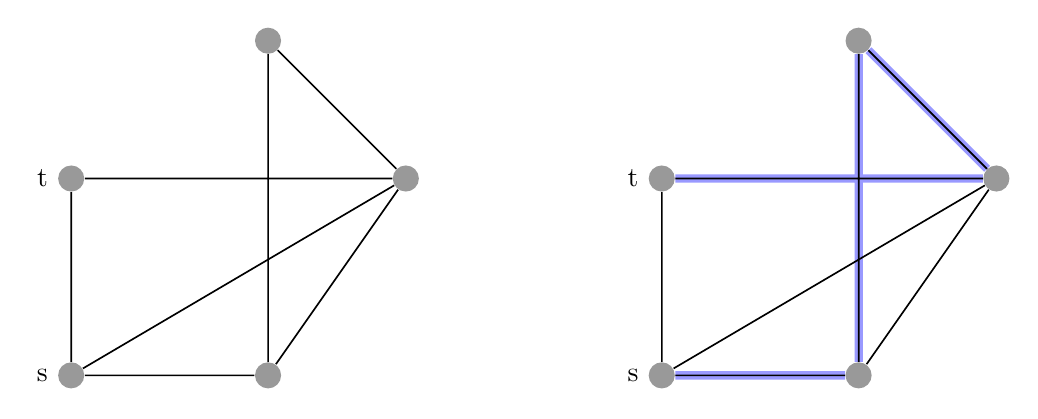
\begin{tikzpicture}
\node (s) at (0,0)[vertex, label=left:s]{};
\node (t) at (0,1)[vertex, label=left:t]{} ;
\node (3) at (1,0)[vertex]{};
\node (4) at (1,1.7)[vertex]{};
\node (5) at (1.7,1)[vertex]{};

% \draw[edgeflow] (s)--(3)--(4)--(5)--(t);
\draw[edge] (s)--(3)--(4)--(5)--(t);
\draw[edge] (t)--(s)--(5)--(3);

%now draw the transformed graph
\node (s2) at (3,0)[vertex, label=left:s]{};
\node (t2) at (3,1)[vertex, label=left:t]{} ;
\node (32) at (4,0)[vertex]{};
\node (42) at (4,1.7)[vertex]{};
\node (52) at (4.7,1)[vertex]{};

\draw[edgeflow] (s2)--(32)--(42)--(52)--(t2);
\draw[edge] (s2)--(32)--(42)--(52)--(t2);
\draw[edge] (t2)--(s2)--(52)--(32);
\end{tikzpicture}
\caption{This graph has an $s-t$-hamilton path contained, marked in blue in the second picture}
\label{bild:hampath}
\end{figure}

An $s-t$-Hamiltonian Path is a path in a network starting at node $s$ and ending at node $t$ that is visiting every 
node of $G$ exactly once like in the example in figure \ref{bild:hampath}. 

This can only work in connected graphs, so we know that if $n$ is the number of nodes in the 
graph, the Hamiltonian Path has to have size $n-1$. Our reduction is the following:

Transform the $s-t$-Hamiltonian Path instance into an instance of a flow network where for each edge $\{uv\}$ there 
are two directed arcs $(u,v),(v,u)$, the arcs $a\in A$ all have capacities $c(a)=[0,1]$ and costs of $-1$ 
with the same underlying graph as before. The nodes $s$ and $t$ become the source and sink of the flow.
The decision we ask for is whether there is a flow with total costs of at most $-(n-1)$ or not. (Figure 
\ref{bild:hampathreduct} shows an example of such a transformation)

 
\begin{figure}[h!]
\centering
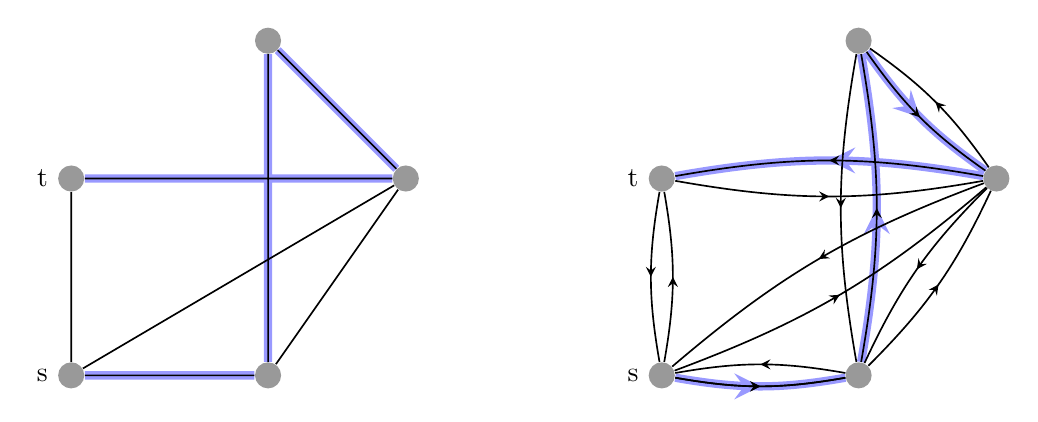
\begin{tikzpicture}
\node (s) at (0,0)[vertex, label=left:s]{};
\node (t) at (0,1)[vertex, label=left:t]{} ;
\node (3) at (1,0)[vertex]{};
\node (4) at (1,1.7)[vertex]{};
\node (5) at (1.7,1)[vertex]{};

\draw[edgeflow] (s)--(3)--(4)--(5)--(t);
\draw[edge] (s)--(3)--(4)--(5)--(t);
\draw[edge] (t)--(s)--(5)--(3);

%now draw the transformed graph
\node (s2) at (3,0)[vertex, label=left:s]{};
\node (t2) at (3,1)[vertex, label=left:t]{} ;
\node (32) at (4,0)[vertex]{};
\node (42) at (4,1.7)[vertex]{};
\node (52) at (4.7,1)[vertex]{};

\draw[curvedarcflow](s2)to(32);
\draw[curvedarcflow](32)to(42);
\draw[curvedarcflow](42)to(52);
\draw[curvedarcflow](52)to(t2);
\draw[curvedarc](s2)to(32);
\draw[curvedarc](32)to(s2);
\draw[curvedarc](42)to(32);
\draw[curvedarc](32)to(42);
\draw[curvedarc](42)to(52);
\draw[curvedarc](52)to(42);
\draw[curvedarc](t2)to(52);
\draw[curvedarc](52)to(t2);
\draw[curvedarc](s2)to(32);
\draw[curvedarc](s2)to(52);
\draw[curvedarc](52)to(s2);
\draw[curvedarc](52)to(32);
\draw[curvedarc](32)to(52);
\draw[curvedarc](t2)to(s2);
\draw[curvedarc](s2)to(t2);

\end{tikzpicture}
\caption{A graph with an $s-t$-hamilton path is transformed to an acyclic minimum cost flow instance with costs of $-1$ 
per arc. Hence in this example we find a minimum acyclic flow of cost $-4=-n+1$}
\label{bild:hampathreduct}
\end{figure}

It is obviously a polynomial time transformation because only a linear number of flags and arcs is added to the 
network, while the edges are deleted when they get replaced with the new arcs.

It yields the same decision as the original Hamiltonian Path instance:
\begin{itemize}
 \item $\Rightarrow:$ Given an instance of the Acyclic Min Cost Flow which has a acyclic flow from $s$ to $t$ with cost 
$-n+1$.
Flow can have a value of at most $1$ on each arc, so each arc the flow is going through can only contribute up to $-1$ 
costs to the cost function. The flow could be split up into different paths from $s$ to $t$, but we know that there are 
no cycles. That means on every of these paths every node is visited only once - if we see it twice we have closed a 
cycle. The cost of the flow is minus the average length of the paths of flow. So we can conclude there is at least one 
path with length $n-1$ that is seeing no node twice - hence it has to see every node exactly once, so we found (at 
least) one $s-t$-Hamiltonian Path and know it is a yes-instance of Hamiltonian Path too.

\item $\Leftarrow:$ Given a graph together with an $s-t$-Hamiltonian Path. In the transformed instance of Min Cost Flow 
we get immediately a feasible $s-t$-Flow by setting the flow value on all forward arcs on the given hamiltonian path 
equals $1$. This flow also has total costs of $-(n-1)$.
\end{itemize}
\end{proof}

These two lemmas together show that our problem of finding an acyclic flow with minimum costs and arbitrary weight 
function is in general $\mathcal{NP}$-complete.
\end{proof}

\newpage
\section{Models and Solving Approaches}%main section about the different models 



\subsection{MIP Formulations}
For many combinatorial Problems it is the best practical solution to formulate them as a Mixed Integer Problem and just 
solve this problem with modern MIP Solvers such as CPlex or Gurobi. Often there are different possible formulations as 
MIP, which might yield very different running times due to numerical or algorithmical reasons. In our problem, it is 
easy to model the flow conservation and the ingoing and outgoing flow on vertices. Like described before, we can assign 
a negative weight to an arc variable and this way maximize flow over this arc by minimizing the overall cost. This 
would be the typical MIP formulation of a min cost flow:

\begin{align*}
  &\min \sum_{a\in A} w_a\cdot x_a  \\
  %TODO an die balance-intervall formulierung anpassen
 s.t. & \sum_{a\in \delta^+(v)}x_a - \sum_{a\in\delta^- (v)}x_a = d_v\ &\forall v\in V \\
  & c_l(a)\le x_a \le c_u(a) & \forall a\in A
\end{align*}

This model still allows cyclic flow, so we have to find constraints to avoid cyclicity. 
\subsubsection{Model 1: Node Potentials}
%TODO welche formulierungen koennte es noch geben fuer dieses problem?
%TODO PORTA results and polytope of the problem?

Another idea (that is unfortunately not a linear formulation anymore) would be to set potentials on he nodes and allow 
only flow from higher to lower potential. This is quite close to reality, where gas will only flow from places wih high 
pressure to places with lower pressure in the network. So each vertex $v$ would become a variable $\pi_v$, each arc $a$ 
as before a variable $x_a$ for the amount of flow. We have to ensure that the values of the potentials are all 
different, or that there is no flow between nodes of the same potential. Otherwise any solution where all potentials 
are set to the same value would fulfill this constraint, regardless if it is acyclic or not. So in pracicewe could set 
a very small constant $\varepsilon > 0$ to describe the minimum distance between the potentials. A feasible solution 
now has to fulfill $$x_a\cdot (\pi_v -\pi_w)\ge 0\,\forall a=(v,w)\in A$$

We get the Mixed Integer Nonlinear Program
\begin{align*}
  &\min \sum_{a\in A} w_a\cdot x_a & \\
 s.t. & \sum_{a\in \delta^+(v)}x_a - \sum_{a\in\delta^- (v)}x_a &=& b_v\ &\forall v\in V \\
 & x_a &\le& c_u(a) & \forall a\in A\\
 & -x_a &\le& c_l(a) & \forall a\in A\\
 & -x_a\cdot (\pi_vx -\pi_w)&\le& 0 &\forall a=(v,w)\in A\\
 & (\pi_v - \pi_w)^2 &\ge& \varepsilon &\forall v,w \in V\\
 & x_a \in \R & & &\forall a\in A\\
 & \pi_v \in \R & & & \forall v\in V\\
 & d_a \in \{0,1\} & & &\forall a\in A\\
\end{align*}

We show that this flow indeed is an acyclic one:

\begin{prop}
 A flow which fulfills the constraints of the above nonlinear program is always acyclic.
\end{prop}
\begin{proof}
 Assume a flow fulfilling the above constraints would have cyclic flow on a cycle $C$. Without loss of generality 
we number the vertices on the cycle from $1$ to $n$ and assume all arcs are directed forward on this cycle. This means 
there are arcs $a_1=(v_1,v_2),a_2=(v_2,v_3), \dots a_n=(v_n, v_1)\in C$ such that $x_{a_i} > 0 \,\forall i={1,\dots , 
n}$. Also we know from the constraints  $x_a\cdot (\pi_v -\pi_w)\ge 0$ and $\pi_v - \pi_w \neq 0$ (Hence $\Rightarrow 
\pi_v\neq\pi_w)\, \forall v,w\in V$. So we conclude an ordering of the vertices potentials: $x_{a_1}\cdot (\pi_{v_1} 
-\pi_{v_2})\ge 0 \Rightarrow \pi_{v_1}>\pi_{v_2}$ and so on. This yields a sequence $\pi_{v_1}>\pi_{v_2}>\dots 
>\pi_{v_n}>\pi_{v_1}$, which is a contradiction. \Lightning
\end{proof}

\subsubsection{Model 2: Acyclicity Constraints On All Cycles}

One idea (which was implemented in Lamatto by Robert Schwarz) is the following: Every arc has a direction and the sign 
of the flow on this arc tells us in which direction flow is send over this arc. Hence we can introduce variables 
$d_a\in 
\{0,1\}$ for each arc $a\in A$ that indicate the direction of flow and are coupled with the flow variables:
\begin{align*}
d_a=1 & \Rightarrow x_a\ge 0 \\
d_a=0 & \Rightarrow x_a\le 0
\end{align*}
These indicator constraints can be handled the way they are by standard MIP solvers, but to make them real MIP 
constraints we have to formulate them as follows (with $M$ a constant bigger than any possible $x_a$ , e.g. 
$M=\sum_{v\in V}|b_v|$) :
\begin{align*}
 x_a + M\cdot (1-d_a) &\ge 0\\
 x_a - M\cdot d_a & \le 0
\end{align*}



Now we have decision variables for the flow direction, we add constraints to avoid cycles. There should be at least 
one arc in each direction, so we get $$ 1\le\sum_{a\in C\textrm{ forward }} d_a + \sum_{a\in C\textrm{ backward 
}}1-d_a\le n-1$$
Let us formulate this in a slightly different way to get only one sum: For each cycle of size $C_n=C_l+C_m$ 
let $C_m$ be the number of arcs directed forward and $C_l$ the number of backward directed arcs. We define that always 
$C_l\le C_m$, so forward is defined as the direction where more arcs are pointing towards (left or right would only 
make 
sense in a planar embedding). Then we get the constraint $$1-l \le \sum_{a\in C}d_a\le n-(l+1)$$ that forbids any
cyclic flow on $C$. We will show later under which conditions such constraints also forbid cyclic flow on other cycles. 
%TODO was ist wenn gleich viele? Ist das als Definition so ueberhaupt ok?

So our MIP formulation of the model is finally
\begin{align*}
 &\min \sum_{a\in A} w_a\cdot x_a & \\
 s.t. & \sum_{a\in \delta^+(v)}x_a - \sum_{a\in\delta^- (v)}x_a = b_v\ &\forall v\in V \\
  & c_l(a)\le x_a \le c_u(a) & \forall a\in A\\
 &x_a + M\cdot (1-d_a) \ge 0 & \forall a\in A\\
 &x_a - M\cdot d_a \le 0 & \forall a\in A\\
 &1-l \le \sum_{a\in C}d_a \le n-(l+1) & \forall \textrm{ cycle }C\in G\\
 & x_a \in \R &\forall a\in A\\
 & d_a \in \{0,1\} &\forall a\in A
\end{align*}
or with only $\le$ inequalities:
\begin{align}
 &\min \sum_{a\in A} w_a\cdot x_a & \\
 s.t. & \sum_{a\in \delta^+(v)}x_a - \sum_{a\in\delta^- (v)}x_a &=& b_v\ &\forall v\in V \\
 & x_a &\le& c_u(a) & \forall a\in A\\
 & -x_a &\le& c_l(a) & \forall a\in A\\
 &-x_a - M\cdot (1-d_a) &\le& 0 & \forall a\in A\\
 &x_a - M\cdot d_a &\le& 0 & \forall a\in A\\
 &1-l - \sum_{a\in C}d_a &\le& 0 & \forall \textrm{ cycle }C\in G\\
 & \sum_{a\in C}d_a +(l+1)-n &\le& 0 & \forall \textrm{ cycle }C\in G\\
 & x_a \in \R & & &\forall a\in A\\
 & d_a \in \{0,1\} & & &\forall a\in A
\end{align}
%TODO gibt es noch andere Möglichkeiten als die von Robert? bestimmt!?



\subsection{The number of cycles we have to forbid}

\newpage
\subsection{A Path-Based Heuristic Approach}
\newpage
\section{Implementation and Computational Results}% The models we described have also been implemented and tested on networks of different size.
In this section we will discuss the practical implementations and present results of the computation. For relevant 
real-world problem sizes the exact models are too slow, even with separation of the acyclicity constraints. For this 
reason we also describe how to relax the problem in order to get useable (though in general not optimal) results for the 
flow bounds. 
We compare the bounds found by different approaches and with different settings (different networks and nominations) 
to see which approach is suited best to actually compute acyclic flow bounds in a network. We also describe in short 
how the standard bounds we used to compare the results to are computed. 

At last we compare the impact of bounds and the number of fixed variables fed into the solver on the model sizes of the 
discretization. \\

\subsection{Implemented Algorithms}

We described the theoretical backgrounds of different algorithms to obtain flow bounds for our problem. The 
computational results of different implementations of them may vary widely, and the performance is influenced by lots 
of details regarding the machines, programming languages, data structures or just code quality. Nevertheless we want 
to give an overview what worked well in the implementation and what did not.\\

All algorithms where tested on a PC with instances of the \textit{"gaslib"} gasnet test library. The library can be 
downloaded on \url{http://gaslib.zib.de/}. A detailed description of this problem library can be found in 
\cite{HumpolaJoormannOucherifPfetschScheweSchmidtSchwarz:2015}.
%TODO muss ich den PC mit Anzahl kernen etc spezifizieren?!?

\subsubsection{MIP with Node Potentials and Binary Direction Variables}
The MIP model described in \ref{model:nodePotential} was implemented in Lamatto, using Gurobi as solver for this 
model. However,the two layers of indicator constraints seem to be a heavy problem of the model in 
practice. The following model was implemented:
\begin{align*}
  &\min \sum_{a\in A} w_a\cdot q_a & \\
 s.t. & \sum_{a\in \delta^+(v)}q_a - \sum_{a\in\delta^- (v)}q_a &=& d_v\ &\forall v\in V \\
 & q_a &\le& c_u(a) & \forall a\in A\\
 & q_a &\ge& c_l(a) & \forall a\in A\\
 & \rho_{vw}=1 &\Rightarrow &\pi_v\ge\pi_w +1 & \forall (v,w)\in A\\
 & \rho_{vw}=0 &\Rightarrow &\pi_w\ge\pi_v +1& \forall (v,w)\in A\\
 & \rho_{vw}=1 &\Rightarrow &q((v,w))\ge 0& \forall (v,w)\in A\\
 & \rho_{vw}=0 &\Rightarrow &q((v,w))\le 0& \forall (v,w)\in A\\
 & q_a \in \R & & &\forall a\in A\\
 & \pi_v \in \R & & & \forall v\in V\\
 & d_a \in \{0,1\} & & &\forall a\in A\\
 & \rho_{vw} \in \{0,1\}&&& \forall a=(v,w)\in A\\
\end{align*}
Integer node potentials imply the direction of the arc between the incident nodes. These binary direction 
variables again imply the sign of the actual flow on an arc. Indicator constraints are usually implemented via 
Big-M-constraints of the form 
\begin{align*}
 &\pi_v-\pi_w &\ge & N(\rho_{vw}-1)+1\\
 &\pi_v-\pi_w&\le &N\rho_{vw}-1 \\
 &q((v,w))&\ge& M(\rho_{vw}-1)\\
 &q((v,w))&\le & M\rho_{vw}\\
 &\rho_{vw} \in \{0,1\}&&\\
\end{align*}
with sufficient big values for $M$ and $N$. This model heavily relies on the Big-M constraints.
For any MIP solver these indicator or Big-M constraints are difficult to handle, because the optimal vertex of the LP 
polyhedron can be quite far from the optimal mixed integer solution.\\

The model was tested on the smallest network named "gaslib-40" of the gaslib package. After running the algorithm for 5 
seconds the optimal bounds for all arcs of the network were computed. The results were the same as with the Acyclicity 
Constraint (separation) Model, apart from numerical rounding differences. \\

On the medium size network "gaslib-135" of the gaslib package TODO

%TODO testergebnisse (vermutlich fail nach etlichen tagen)

\subsubsection{MIP with Binary Direction Variables and separated Acyclicity Constraints}
In section \ref{model:AcyclicityConstraints} we described a model using acyclicity constraints on the binary directions 
for each cycle that was found during the solving process.
This model itself is independent of the implementation of the acyclicity constraints. But since a graph can have an 
exponential number of cycles, writing down all constraints of the model alone could take exponential time. The 
model redundancies we described in \ref{prop:redundantAcyclicityCons} are not enough to sufficiently reduce the model 
size - in fact it could happen that the conditions for \ref{prop:redundantAcyclicityCons} do not apply at all in 
certain networks (though we also did not proof that a clever generalization of the proposition couldn't do better). 
For example the condition of the proposition states that there have to be two cycles with exactly one arc in common. 
But there are of course example networks not containing any two cycles like this. (You could just subdivide every arc 
in a network. Then every two cycles have at least two arcs in common.)\\

So the implementation does not add all the acyclicity constraints explicitely. Instead, the MIP Solver gets a 
general constraint that demands that there is no cyclic flow in the network. When this constraint is checked and there 
is cyclic flow somewhere in the network, a new linear acyclicity constraint on the cycle with the detected cyclic flow 
is added. An Acyclicity Constraint Handler was implemented for this thesis in Lamatto with SCIP as MIP solver. \\

Like the other exact model with node potentials this model takes lots of time to compute the optimal solution. In 
a network there are huge numbers of arcs to be computed that yield similar subproblems, some of them being 
difficult and running very long. Like in the Node Potential Model we could only produce an exact solution for the 
"gaslib-40" network while the algorithm was running too long on the other gaslib test instances.

\subsubsection{Relaxations of the Exact Separation Model}
If we want to have fast answers or compute bigger networks the exact model with separation of acyclicity 
constraints does not work in practice. Nevertheless this model gives us an interesting relaxation of the acyclic 
flowbound problem for free: 

We can limit the time or the number of nodes in the branch and bound tree for each arc in the network. If an optimal 
solution can be found with low effort, we get the optimum bound. If the situation is difficult and we run into the limit 
we just take the dual bound of the mixed integer program. This number is always an upper bound because it is always 
greater or equal to the optimum (which is the maximum flow). \\

With this algorithm we will always get some solution. This solution might be $\infty$. To get rid of the infinite 
values, we can combine it with a simple bound estimate. For example we can take the sum of all ingoing flow as upper 
bound for all arcs with a dual bound that is greater than this. Depending on the preset limit this dual solution could
closer to or further from the optimum. 

This relaxation was implemented with a limit on the nodes and is compared to 
others in the tables below. The tables refer to this relaxation as "sepa\_X" for the exact MIP with separation of 
acyclicity constraints and a node limit of \textit{X} in the branch and bound process of the MIP.

\subsubsection{Acyclicity Constraints on a Cycle Base}% this is roberts code, props to him!
This idea was the starting point of this thesis and implemented by Robert Schwarz some time before. It is like the 
former an incomplete application of the acyclicity constraints. It adds all its acyclicity constraints in the 
beginning. The advantages are easier implementation and hope for a faster running time since the solver does not need 
to add new constraints all the time.

We have seen in \ref{bild:reichtkreisbasis2} that the acyclicity constraints of a small subset of the cycles (like a 
cycle base) do not suffice to forbid cyclic flow  in the network. Still we can try to use them as a relaxation to the 
exact problem. This will already avoid cyclic flow on single cycles that are not touching each other. The tables show 
how the idea works out in practice.

\subsubsection{Cyclic Flow Bounds}%describe the exactfb algo implemented before
\label{model:cyclicFlow}
To start a comparison we need a bound value to which we can compare. This value should be one that is fast and 
easy to compute, in some way sensible and not too far away from a realistic solution, and of course a valid upper 
bound. 
One of the first algorithmic problems that one might think of after seeing the flowbound problem is the normal minimum 
cost flow problem \ref{def:mincostflow}. Setting a negative weight on only one arc in the network will 
maximize flow on this specific arc. We described the connections with this problem in section \ref{sect:mincostflow}. 

We can set the maximal flow capacity on an arc to the natural upper bound "sum of all ingoing flow" if no tighter 
capacity bounds are given. This is a very easy condition derived from the acyclicity and can always be applied.

This model is also implemented in Lamatto. It is modeled as a mixed integer programm with only flow balance and 
capacity constraints. Binary directions are not contained in this model. Because this MIP model also served as the 
basis for the more specific MIP models it is a relaxation of all the others which just add some more constraints or 
variables.

We will refer to this model as "cyclic bounds" respectively "cyclic bounds + flowsum" in the tables below. We compare 
the bounds from the different algorithms to the bounds found with this approach. 


\subsubsection{Tables}
\begin{center}

\begin{tabular}{ l | c | c | c | c }
\textbf{gaslib-40} & Time  & Fixed Flows & Bounds tightened & avg improvement\\
\hline
 cyclic bounds& $<1s$ & 21 & [-48] & [-7825.0] \\
 cyclic bounds+flowsum& $<1s$ & 21 & - & - \\
 cycle base& $1s$ & 21 & 48 & 1372.4\\
 heuristic& $<1s$& 21& 0 & 0\\
 node potential& $4s$ & 21 & 48 & 1372.4 \\ 
 sepa\_all& $112s$ & 21 & 48 & 1372.4\\
\end{tabular} 
\end{center}
%ergebnisse fuer 135: nodepotential hatte gerade einmal das erste pipe berechnet (600) mit beiden schranken, nach 293 h 
%rechenzeit, sepa (auf nur einem kern aber im gleichen rechner) war ebenfalls nicht fertig

\begin{center}
\begin{tabular}{ l | c | c | c | c }
\textbf{gaslib-582 warm\_1111} & Time  & Fixed Flows & Bounds tightened & avg improvement \\
\hline
%  cyclic bounds& $<1s$ & 21 & [-48] & [-7825.0] \\
 cyclic bounds+flowsum& $1s$ & 365 & - & -\\
 cycle base& $ $ &  &  &\\
 heuristic& $ 11s$& 365& 164 & 5047.2 \\
 node potential& $ $ &  &  &   \\ 
 sepa\_1000& $ 50 min$ & 382 & 107 & 3802.1 \\
 sepa\_5000& $ 159 min$ & 382 & 180 & 3971.6 \\
 sepa\_20000& $ 281 min$ & 382 & 264 & 4312.5 \\
 sepa\_60000& $702 min $ & 382& 278& 4267.7\\
\end{tabular} 
\end{center}

\begin{center}
\begin{tabular}{ l | c | c | c | c }

\textbf{gaslib-582 cool\_12} & Time  & Fixed Flows & Bounds tightened & avg improvement\\
\hline
%  cyclic bounds& $<1s$ & 21 & [-48] & [-7825.0] \\
 cyclic bounds+flowsum& $1s$ & 365 & - & - \\
 cycle base& $ $ &  &  & \\
 heuristic& $11s $& 365 & 164 & 4050.9 \\
 node potential& $ $ &  &  &    \\ 
 sepa\_1000& $ 50 min $ & 378 & 100 & 3025.2\\
 sepa\_5000& $ 158 min$ & 378 & 211 & 3525.6\\ 
 sepa\_20000& $ 361 min$ & 378 & 242 & 3648.3  \\
 sepa\_60000& $678 min $ & 378 & 276 & 3390.3 \\
\end{tabular} 
\end{center}

\begin{center}
\begin{tabular}{ l | c | c | c | c }

\textbf{gaslib-582 cold\_100} & Time  & Fixed Flows & Bounds tightened & avg improvement\\
\hline
%  cyclic bounds& $<1s$ & 21 & [-48] & [-7825.0] \\
 cyclic bounds+flowsum& $1s$ & 365 & - & -  \\
 cycle base& $ $ &  &  & \\
 heuristic& $ 10s $& 365& 164 & 5157.4\\
 node potential& $ $ &  &  &   \\ 
 sepa\_1000& $50 min $ & 378 & 88 & 4265.5 \\
 sepa\_5000& $ 127 min$ & 378 & 242 & 4508.9  \\
 sepa\_20000& $ 382 min$ &  378& 241 & 4526.3  \\
 sepa\_60000& $635 min $ & 378& 283& 4200\\
\end{tabular} 
\end{center}

\begin{center}
\begin{tabular}{ l | c | c | c | c }

\textbf{gaslib-582 freezing\_1} & Time  & Fixed Flows & Bounds tightened & avg improvement\\
\hline
%  cyclic bounds& $<1s$ & 21 & [-48] & [-7825.0] \\
 cyclic bounds+flowsum& $1s$ & 365 & - & - \\
 cycle base& $ $ &  &  & \\
 heuristic& $ 11s$& 365& 148 & 6148.2\\
 node potential& $ $ &  &  &  \\ 
 sepa\_1000& $50 min $ & 374 & 90 & 5405.4 \\
 sepa\_5000& $ 154 min$ & 374 & 231 &5104  \\
 sepa\_20000& $366 min $ & 374 & 244 &4929.8 \\
 sepa\_60000& $593 min $ & 374& 276& 4777.6\\
\end{tabular} 
\end{center}

\begin{center}
\begin{tabular}{ l | c | c | c | c }

\textbf{gaslib-582 mild\_10} & Time  & Fixed Flows & Bounds tightened & avg improvement\\
\hline
%  cyclic bounds& $<1s$ & 21 & [-48] & [-7825.0] \\
 cyclic bounds+flowsum& $1s$ & 365 & - & -\\
 cycle base& $ $ &  &  & \\
 heuristic& $11s $&365 & 164 & 4291.5\\
 node potential& $ $ &  &   &  \\ 
 sepa\_1000& $50 min $ & 378 & 105 & 3271.3 \\
 sepa\_5000& $ 158 min $ & 378 & 188 & 3329.5 \\
 sepa\_20000& $ 394 min$ & 378 & 216 &3144.6 \\
 sepa\_60000& $651 min $ & 378& 289&3593.3 \\
\end{tabular} 
\end{center}

The results show that in all cases the bounds get better with more time for the separation algorithm, while the exact 
models need too much time. The heuristics results are weak, but far better than setting the limit to only 1000 nodes. 
%TODO mehr schreiben hier
The bounds computed can be read in and used by the solver to improve building of other models like the discretization. 
The impact of the computed flow bounds on this model is shown in the tables below.

\begin{center}
\begin{tabular}{ l | c | c | c | c |c}

\textbf{gaslib-582 cold\_100} & Modelbuilding Time  & Fixed Dirs & nonlinear f. & vars(cont,disc)&cons\\
\hline
%  cyclic bounds& $<1s$ & 21 & [-48] & [-7825.0] \\
 cyclic bounds+flowsum& $7s$ & 440/609 & 241(219+22)& 5727(4113+1614)&8216 \\
%  cycle base& $ $ &  &  & \\
 heuristic& $ 8s$& 440/609& 241(219+22) & 5675(4087+1588)&8162\\
%  node potential& $ $ &  &  &  \\ 
 sepa\_1000& $7s $ & 467/609 & 237(217+20)& 5471(3977+1944) & 7930 \\
 sepa\_5000& $ 7s$ & 467/609& 237(217+20)& 5185(3834+1351)&7641  \\
 sepa\_20000& $7s$& 467/609 & 237(217+20) & 5185(3834+1351)& 7640 \\
 sepa\_60000& $ 8s$& 469/609 &237(217+20) & 4903(3693+1210)& 7339 \\
\end{tabular} 
\end{center}



\newpage
\section{Summary}




\newpage
\newpage
\addcontentsline{toc}{section}{Bibliography}
\bibliographystyle{amsplain}
% \bibliographystyle{apalike}
\bibliography{literatur}
\nocite{*}

\end{document}
